% !TEX root = ../intro-stellar-physics.tex

\newcommand*{\Pl}[1]{\ensuremath{\mathcal{P}_{#1}}}

You may recall from electrostatics that we can decompose the field from a set of charges into a sum of moments: dipole, quadrupole, and so on. The basis functions for this are the Legendre polynomials $\Pl{n}(\cos\theta)$, defined by the expansion
\begin{equation}
	\frac{1}{\sqrt{1 - 2xz + z^{2}}} = \sum_{n=0}^{\infty}\Pl{n}(x)z^{n},
\end{equation}
for $-1<x<1,\;|z| < 1$. The first three polynomials are
\begin{eqnarray}
	\Pl{0}(x) &=& 1 \nonumber\\
	\Pl{1}(x) &=& x \nonumber\\
	\Pl{2}(x) &=& \frac{1}{2}(3x^{2}-1).
\end{eqnarray}
The first eight Legendre polynomials are plotted below.

\begin{figure*}
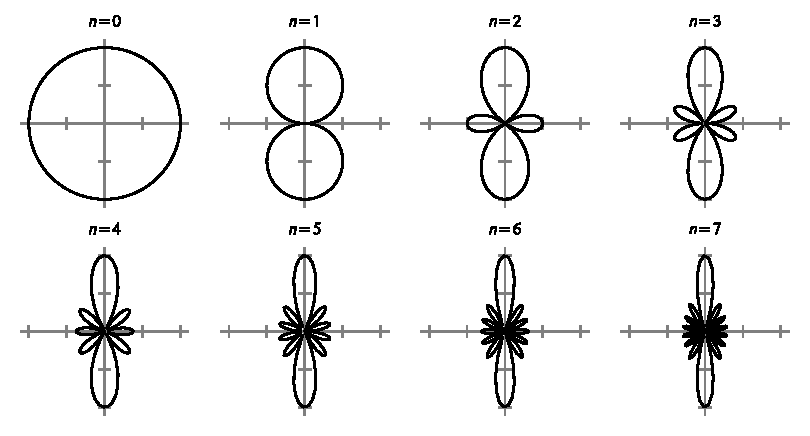
\includegraphics[width=\linewidth]{legendre}
\caption[Legendre polynomials]{\label{f.legendre}
Polar plots of $\Pl{n}(\cos\theta)$ for $n=0,\ldots,7$.}
\end{figure*}

The Legendre polynomials are \emph{orthogonal} in the following sense:
\begin{equation}\label{e.orthogonal}
\int_{-1}^{1}\Pl{n}(\mu)\Pl{m}(\mu)\dif \mu = \left\{
\begin{array}{lr}
	0 &  m\neq n\\
	\frac{2}{2n+1} & m=n
\end{array}\right..
\end{equation}
As a result, we can decompose the radiative intensity into multipoles:
\begin{equation}\label{e.decomposition}
	I = \sum_{n=0}^{\infty} I_{n} \Pl{n}(\mu).
\end{equation}
As $n$ increases, the angular scale of variations becomes finer.

\newthought{To take moments of the intensity}, notice that we can write the weighting factors in terms of Legendre polynomials:
\begin{eqnarray*}
	J &=& \frac{1}{4\pi}\int\,\dif\phi\dif\mu\,{\color{red}\mu^{0}}\,I 
		= \frac{1}{2}\int_{-1}^{1}\dif\mu\sum_{n=0}^{\infty} \,{\color{red}\Pl{0}} I_{n} \\
	H &=& \frac{1}{4\pi}\int\,\dif\phi\dif\mu\,{\color{red}\mu^{1}}\,I 
		= \frac{1}{2}\int_{-1}^{1}\dif\mu\sum_{n=0}^{\infty} \,{\color{red}\Pl{1}} I_{n} \\
	K &=& \frac{1}{4\pi}\int\,\dif\phi\dif\mu\,{\color{red}\mu^{2}}\,I 
		= \frac{1}{2}\int_{-1}^{1}\dif\mu\sum_{n=0}^{\infty} \,{\color{red} \frac{1}{3}(2\Pl{2}+\Pl{0})} I_{n}
\end{eqnarray*}
Now we can use the orthogonality relation (eq.~[\ref{e.orthogonal}]) to compute the integrals:
\begin{eqnarray*}
	J &=& I_{0} \\
	H &=& \frac{1}{3}I_{1} \\
	K &=& \frac{1}{3}\left(\frac{2}{5}I_{2} + I_{0}\right)
		= \frac{1}{3}\left(\frac{2}{5}I_{2} + J\right)
\end{eqnarray*}
Applying the Eddington approximation, i.e., setting $K = J/3$, means that we must set $I_{2} = 0$. Once we do this, we can solve for $J$, $H$, and $K=J/3$ as functions of optical depth $\tau$. This gives us a description of the radiative intensity in terms of $J(\tau)$ and $H$,
\[
	I(\tau,\mu) = J(\tau) + 3H \Pl{1}(\mu) + \cdots \approx J(\tau) + 3H\cos\theta,
\]
which neglects the higher order terms $I_{n}\Pl{n},\forall n > 2$.
